% !TEX program = xelatex
\documentclass[10pt,letterpaper,twocolumn]{article}

% === GEOMETRY ===
\usepackage[top=0.75in, bottom=0.75in, left=0.75in, right=0.75in]{geometry}

% === FONTS ===
\usepackage{fontspec}
\setmainfont{Latin Modern Roman}[
  Extension=.otf,
  UprightFont=lmroman10-regular,
  BoldFont=lmroman10-bold,
  ItalicFont=lmroman10-italic,
  BoldItalicFont=lmroman10-bolditalic,
]
\setsansfont{Latin Modern Sans}[
  Extension=.otf,
  UprightFont=lmsans10-regular,
  BoldFont=lmsans10-bold,
  ItalicFont=lmsans10-oblique,
  BoldItalicFont=lmsans10-boldoblique,
]
\setmonofont{Latin Modern Mono}[
  Extension=.otf,
  UprightFont=lmmono10-regular,
  ItalicFont=lmmono10-italic,
  Scale=0.85,
]
% YWFT Processing carries the display title only. Its punctuation glyphs
% are unreliable and its charset omits dashes, so nothing with a mark in
% it is ever set in this face.
\newfontfamily\acbold{ywft-processing-bold}[
  Path=../../system/public/type/webfonts/,
  Extension=.ttf
]

% === PACKAGES ===
\usepackage{xcolor}
\usepackage{titlesec}
\usepackage{enumitem}
\usepackage{booktabs}
\usepackage{tabularx}
\usepackage{fancyhdr}
\usepackage{hyperref}
\usepackage{xurl}
\usepackage{graphicx}
\usepackage{ragged2e}
\usepackage{microtype}
\usepackage{natbib}
\usepackage{tikz}
\usetikzlibrary{positioning,arrows.meta,calc,shapes.geometric}
\usepackage{../ac-source-bundle}

% === COLORS ===
\definecolor{acpink}{RGB}{180,72,135}
\definecolor{acpurple}{RGB}{120,80,180}
\definecolor{acdark}{RGB}{64,56,74}
\definecolor{acgray}{RGB}{119,119,119}
\definecolor{acgreen}{RGB}{46,150,72}
\definecolor{acblue}{RGB}{54,110,190}
\definecolor{acamber}{RGB}{201,138,20}

% === HYPERREF ===
\hypersetup{
  colorlinks=true,
  linkcolor=acpurple,
  urlcolor=acpurple,
  citecolor=acpurple,
  pdfauthor={@jeffrey},
  pdftitle={iOS So Far},
}

% === SECTION FORMATTING ===
\titleformat{\section}
  {\normalfont\bfseries\normalsize\uppercase}
  {\thesection.}
  {0.5em}
  {}
\titlespacing{\section}{0pt}{1.2em}{0.3em}
\titleformat{\subsection}
  {\normalfont\bfseries\small}
  {\thesubsection}
  {0.5em}
  {}
\titlespacing{\subsection}{0pt}{0.8em}{0.2em}

% === HEADER/FOOTER ===
\pagestyle{fancy}
\fancyhf{}
\renewcommand{\headrulewidth}{0pt}
\fancyhead[C]{\footnotesize\color{acgray}\textit{iOS So Far}}
\fancyfoot[C]{\footnotesize\thepage}

% === LISTS, COLUMNS, PARAGRAPHS ===
\setlist[itemize]{nosep, leftmargin=1.2em, itemsep=0.15em}
\setlist[enumerate]{nosep, leftmargin=1.4em, itemsep=0.15em}
\setlength{\columnsep}{1.8em}
\setlength{\parindent}{1em}
\setlength{\parskip}{0.3em}
\tolerance=800
\emergencystretch=1em
\hyphenpenalty=50

% === BRAND ===
\newcommand{\acdot}{{\color{acpink}.}}
\newcommand{\ac}{Aesthetic{\acdot}Computer}

% === TIKZ STYLES ===
\tikzset{
  stage/.style={draw=acgray!70, line width=0.5pt, rounded corners=2pt,
                fill=white, inner sep=3.4pt, font=\scriptsize\sffamily,
                text=acdark, minimum height=13pt, align=center},
  flow/.style={-{Stealth[length=3.6pt,width=3pt]}, draw=acgray!75, line width=0.5pt},
  stall/.style={draw=acamber, line width=0.8pt, fill=acamber!8, rounded corners=2pt,
                inner sep=3.2pt, font=\scriptsize\sffamily, text=acdark, align=center},
  ship/.style={draw=acgreen, line width=0.8pt, fill=acgreen!8, rounded corners=2pt,
               inner sep=3.2pt, font=\scriptsize\sffamily, text=acdark, align=center},
  tag/.style={font=\tiny\sffamily, text=acgray, align=left},
}

\begin{document}

\twocolumn[{%
\begin{center}
{\acbold\fontsize{30pt}{34pt}\selectfont\color{acdark} iOS So Far}\par
\vspace{0.55em}
{\itshape\fontsize{13pt}{16pt}\selectfont\color{acpink}
Ten years of \ac{} on Apple's store, read from the record}\par
\vspace{0.6em}
{\small\color{acgray} \href{https://prompt.ac/@jeffrey}{@jeffrey} \,$\cdot$\, \ac{} \,$\cdot$\, ORCID \href{https://orcid.org/0009-0007-4460-4913}{0009-0007-4460-4913}}\par
\vspace{0.25em}
{\small\color{acgray} 9 September 2026}\par
\vspace{0.55em}
{\color{acpink}\rule{\textwidth}{1.2pt}}
\vspace{0.5em}
\end{center}

\begin{quote}
\small\noindent\textbf{Abstract.}
Six app records have accumulated under one Apple developer account since
2016: \emph{Finger Quilt}, \emph{No Paint}, \emph{Soft Wallpaper},
\ac{} for iOS, \emph{Menu Band}, and the unreleased
\emph{oskiewar}. Together they hold 152 lifetime customer reviews
averaging 4.65 stars and have earned \$17.81 in developer proceeds across
five paid units, all sold in a nine-week window of 2026. This paper reads
that record from primary sources: the App Store Connect API, the store's
own analytics reports, the runtime's boot telemetry, and the repository's
commit history. Three findings organize it. First, the only demand event
in ten years arrived from outside the store, when short-video attention
drove 112 reviews of \emph{No Paint} between June and September 2020 and
decayed to nothing within a year. Second, the constraint on the current
portfolio is the last mile rather than production: \ac{} for iOS
booted 13,830 handheld sessions in 2026 while serving a binary
released in July 2023, because two later builds were uploaded, left
unreleased, and allowed to expire. Third, every recorded sale of
\emph{Menu Band} occurred at \$4.99, and the app now lists at \$9.99. I
close with nine ranked openings, each tied to the evidence that
motivates it and the smallest action that would test it.
\end{quote}
\vspace{0.5em}
}]

\section{Introduction}

This is an audit, and it exists because a smaller question had no
answer. Asked in September 2026 whether \emph{Menu Band} had sold any
copies since the last check, the honest reply took a scripted pull
against Apple's analytics API and arrived at five units. Asked the
obvious follow-up, whether the same numbers were available for the other
apps, the answer was that they were not, because no analytics report had
ever been requested for any of them. Ten years of store presence had
produced no measurement apparatus at all.

That gap is the subject. \ac{} is a runtime and social network for
creative computing whose principal surface is a URL~\citep{scudder2026ac}.
Its native surfaces have grown alongside it: a web wrapper for iPhone, a
menu-bar instrument for macOS~\citep{scudder2026notepat}, a native
operating system for handheld hardware~\citep{scudder2026os}. Apple's
store is one distribution channel among several, and it is the only one
that reports back. What it reports is worth reading carefully, because
the sums involved are small enough that every individual event is legible.
Five transactions can be examined one at a time. One hundred thirty-one
reviews can be read in full. This is an unusual condition for a
distribution audit, and it makes conclusions available that a larger
dataset would only average away.

Three questions structure the paper. What is actually in the record?
Where did the demand that appeared in it come from? And given both, what
is the smallest set of actions that would change the next ten years?
Sections~\ref{sec:method} through~\ref{sec:runtime} answer the first two
from primary evidence. Section~\ref{sec:openings} answers the third as
nine ranked openings.

The paper's posture follows the sustainability thread in the surrounding
research platter~\citep{scudder2026sustainability}, which asks who pays
for creative tools. Here the question narrows to a channel and a decade,
and the finding is specific: the channel has been supplied with software
and starved of the four or five administrative acts that convert software
into distribution.

\section{Method}
\label{sec:method}

Every number in this paper comes from a primary source pulled on
9~September 2026. Nothing is estimated and nothing is taken from a
dashboard screenshot.

\textbf{App Store Connect API.} App records, version histories, build
histories, category and age assignments, price points, and the complete
customer-review corpus were pulled over the REST
API~\citep{apple2026ascapi} using an ES256 JSON Web Token signed with the
account's admin key. The review endpoint returns full text, rating,
territory, and creation date per review, so review counts here are
censuses rather than samples.

\textbf{Analytics reports.} Unit sales come from the App Store Connect
analytics pipeline~\citep{apple2026analytics}, specifically an ONGOING
report request of type \emph{App Store Purchases Standard}. The pipeline
has three properties that shape what can be claimed. Report instances
restate earlier dates, so for each granularity and row date only the
instance with the latest processing date counts. Days without sales
produce no instance, so silence and zero are indistinguishable in the
raw feed and are separated by checking that the request is still
live. And each ONGOING request has a backfill horizon roughly four weeks
before its creation, which for the one existing request is 13~July 2026.
The tally script implementing these rules lives in the repository at
\texttt{slab/menuband/bin/sales-tally.mjs}.

\textbf{Runtime telemetry.} \ac{} writes one document per page load to a
MongoDB collection named \texttt{boots}, carrying user agent, host, path,
screen geometry, language, timezone, and a coarse geographic region. The
iOS application sets the custom user-agent string \texttt{Aesthetic}; its
macOS sibling sets the same string, and the two are separated by screen
geometry, treating a device pixel ratio of two or more together with a
logical width at or below 1024 points as handheld. Boot counts are page
loads. They are not people, and the runtime carries no per-user analytics
by design.

\textbf{Repository history.} Commit counts and first and last touch dates
per application directory come from \texttt{git log} against the
monorepo. Submission narratives come from \texttt{apple/PROGRESS.md},
which records per-build notes written at the time.

The evidence tables sit beside this paper in \texttt{data/}, with a
README recording what is solid, what is soft, and what is missing. Store
listing strings, which are lowercased for some records, are preserved
verbatim in \texttt{data/app-records.csv}; this paper writes every
product name in house style.

\section{The Record}
\label{sec:record}

Table~\ref{tab:records} is the account as it stands. Six app records span
ten years and four bundle-identifier conventions, which is itself a
readable trace of a practice that changed names.

\begin{table*}[t]
\centering
\small
\caption{The six app records, pulled from the App Store Connect API on 9~September 2026. Released versions counts App Store version records that reached distribution. \emph{No Paint} charged roughly \$3 during its 2020 peak and is free today; the API retains only current prices.}
\label{tab:records}
\begin{tabularx}{\textwidth}{@{}l l l l r r X r@{}}
\toprule
\textbf{App} & \textbf{Platform} & \textbf{First release} & \textbf{Last release} & \textbf{Vers.} & \textbf{Price} & \textbf{Category} & \textbf{Reviews} \\
\midrule
No Paint            & iOS          & 2016-04-24 & 2021-08-03 & 7  & free   & Games         & 131 \\
Finger Quilt        & iOS          & 2016-09-11 & 2016-09-15 & 3  & free   & Photo \& Video & 2 \\
Soft Wallpaper      & iOS          & 2018-05-26 & 2018-06-14 & 5  & free   & Utilities     & 17 \\
\ac{} (iOS)  & iOS          & 2023-07-04 & 2023-07-04 & 1  & free   & Games         & 2 \\
Menu Band           & macOS        & 2026-05-07 & 2026-08-25 & 11 & \$9.99 & Music         & 0 \\
oskiewar            & iOS + macOS  & ---        & ---        & 0  & ---    & ---           & 0 \\
\bottomrule
\end{tabularx}
\end{table*}

Read as a shape, the account has two dense periods separated by a long
thin one. Between 2016 and 2018 three small iOS pieces shipped and
stopped. Between 2018 and 2026 one app shipped, once. Then in a single
summer, 2026 produced eleven \emph{Menu Band} releases, a macOS build of
\ac{} for iOS, and a complete \emph{oskiewar} submission
package.

The reception is consistent and positive wherever there is enough of it
to read. Across 152 lifetime reviews the mean rating is 4.65. The
distribution is bimodal in the way small-sample app reviews usually are,
with 133 five-star ratings against nine one-star ratings and almost
nothing between. Reading the nine, three are jokes about the app being
haunted, one is a complaint about a since-changed price, one is a
professional dispute unrelated to the software, and two are genuine
usability failures that recur elsewhere in the corpus. The two are worth
naming because they are actionable: no visible way to start a new
painting, and no undo.

\emph{Menu Band} has zero reviews after eleven releases and five sales,
which is the expected outcome of that sample size rather than a signal.
\emph{No Paint} carries sixteen published developer responses, and at
least one reviewer noticed, opening a 2026 five-star review with delight
that anyone replies at all.

\section{The One Demand Event}
\label{sec:demand}

Figure~\ref{fig:timeline} plots the whole decade on one axis: release
marks per app above, monthly \emph{No Paint} review volume below. The
asymmetry is the paper's first finding. Of 131 reviews collected over ten
years, 112 arrived in four months.

\begin{figure*}[t]
\centering
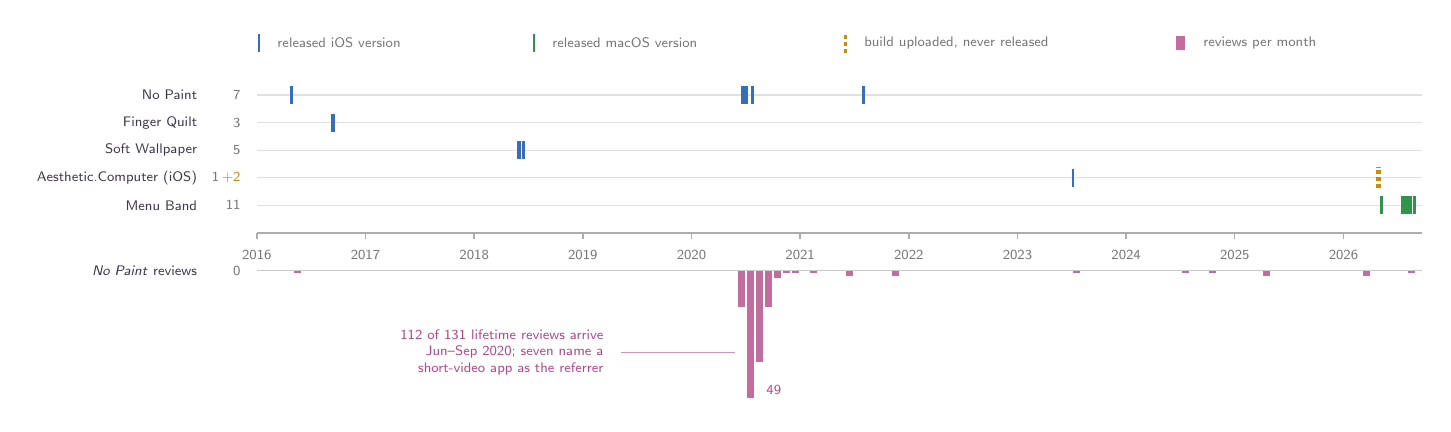
\begin{tikzpicture}[x=1.38cm, y=1cm]

% ================= release lanes =================
% One lane per app. Ticks are individual store releases; the count column
% sits immediately left of the plot so volume compares vertically without
% pushing labels past the text block.
\def\lanA{2.75} \def\lanB{2.40} \def\lanC{2.05} \def\lanD{1.70} \def\lanE{1.35}
\foreach \ry/\lbl/\cnt in {%
  \lanA/No Paint/7, \lanB/Finger Quilt/3, \lanC/Soft Wallpaper/5,
  \lanD/\ac{} (iOS)/{1\,{\color{acamber}+2}}, \lanE/Menu Band/11} {
  \draw[acgray!22, line width=0.4pt] (0,\ry) -- (10.72,\ry);
  \node[font=\tiny\sffamily, text=acdark, anchor=east] at (-0.46,\ry) {\lbl};
  \node[font=\tiny\sffamily, text=acgray, anchor=east] at (-0.06,\ry) {\cnt};
}

% released versions
\foreach \x/\ry in {0.317/\lanA, 4.467/\lanA, 4.469/\lanA, 4.486/\lanA,
                    4.511/\lanA, 4.561/\lanA, 5.586/\lanA,
                    0.697/\lanB, 0.706/\lanB, 0.708/\lanB,
                    2.406/\lanC, 2.419/\lanC, 2.422/\lanC, 2.453/\lanC, 2.456/\lanC,
                    7.511/\lanD}
  \draw[acblue, line width=1.0pt] (\x,\ry-0.115) -- (\x,\ry+0.115);
\foreach \x in {10.353, 10.542, 10.550, 10.567, 10.586, 10.594,
                10.600, 10.608, 10.619, 10.653}
  \draw[acgreen, line width=1.0pt] (\x,\lanE-0.115) -- (\x,\lanE+0.115);
\foreach \x in {10.314, 10.336}
  \draw[acamber, line width=1.0pt, dash pattern=on 1.5pt off 1.0pt]
        (\x,\lanD-0.135) -- (\x,\lanD+0.135);

% ================= time axis =================
\draw[acgray!60, line width=0.5pt] (0,1.00) -- (10.72,1.00);
\foreach \y in {0,1,2,3,4,5,6,7,8,9,10} {
  \draw[acgray!60, line width=0.5pt] (\y,1.00) -- (\y,0.925);
  \pgfmathtruncatemacro{\lab}{\y+2016}
  \node[font=\tiny\sffamily, text=acgray, anchor=north] at (\y,0.905) {\lab};
}

% ================= review volume =================
% Baseline 0.52; 49 reviews maps to 1.62cm.
\def\rs{0.033}
\draw[acgray!40, line width=0.4pt] (0,0.52) -- (10.72,0.52);
\node[font=\tiny\sffamily, text=acdark, anchor=east] at (-0.46,0.52)
  {\emph{No Paint} reviews};
\node[font=\tiny\sffamily, text=acgray, anchor=east] at (-0.06,0.52) {0};
\foreach \m/\n in {0.375/1, 4.458/14, 4.542/49, 4.625/35, 4.708/14, 4.792/3,
                   4.875/1, 4.958/1, 5.125/1, 5.458/2, 5.875/2, 7.542/1,
                   8.542/1, 8.792/1, 9.292/2, 10.208/2, 10.625/1}
  \fill[acpink!80] (\m-0.032,0.52) rectangle (\m+0.032,{0.52-\n*\rs});
% peak label on the tallest bar
\node[font=\tiny\sffamily, text=acpink, anchor=west] at (4.60,{0.52-49*\rs+0.10}) {49};

% spike annotation in the open field to the left
\draw[acpink!60, line width=0.5pt] (4.40,-0.52) -- (3.35,-0.52);
\node[font=\tiny\sffamily, text=acpink, anchor=east, align=right] at (3.28,-0.52)
  {112 of 131 lifetime reviews arrive\\Jun--Sep 2020; seven name a\\short-video app as the referrer};

% ================= legend =================
\draw[acblue, line width=1.0pt] (0.02,3.30) -- (0.02,3.52);
\node[font=\tiny\sffamily, text=acgray, anchor=west] at (0.10,3.41) {released iOS version};
\draw[acgreen, line width=1.0pt] (2.55,3.30) -- (2.55,3.52);
\node[font=\tiny\sffamily, text=acgray, anchor=west] at (2.63,3.41) {released macOS version};
\draw[acamber, line width=1.0pt, dash pattern=on 1.5pt off 1.0pt] (5.42,3.28) -- (5.42,3.54);
\node[font=\tiny\sffamily, text=acgray, anchor=west] at (5.50,3.41) {build uploaded, never released};
\fill[acpink!80] (8.46,3.32) rectangle (8.54,3.50);
\node[font=\tiny\sffamily, text=acgray, anchor=west] at (8.62,3.41) {reviews per month};
\end{tikzpicture}
\caption{Ten years on one axis. Above: every store release, one lane per app, with the release count at the left of each lane. Below: monthly review volume for \emph{No Paint}, the only app with enough reviews to plot. The 2020 spike is the single demand event in the record, and it originated outside the App Store.}
\label{fig:timeline}
\end{figure*}

The reviews say where the attention came from. Seven name a short-video
platform explicitly, one of them naming the \texttt{@whistlegraph}
account directly and instructing readers to go watch the videos that
explain the app. The vocabulary of the spike is consistent and
unprompted: across the corpus, \emph{calming} appears fourteen times,
\emph{relaxing} twelve, \emph{creative} thirteen, \emph{anxiety} five.
Reviewers described a drawing tool they had been handed by a video, and
they described it as a way to feel better.

Three features of the event matter for what follows.

It was external. Nothing in the App Store produced it. The store received
the traffic and converted it, which is a real service, and the store did
not originate it.

It was monetized thinly and then abandoned. Two reviews from the peak
complain about price, one calling roughly \$3 expensive and another
calling it terrible value, which fixes the app as paid during its most
visible months. It is free today. The last release shipped in August
2021, twelve months after the peak, and nothing has shipped since.

It decayed completely. Review volume fell from 49 in July 2020 to three
in October 2020 and to single digits per year thereafter. The audience
was acquired and not retained, and no mechanism existed to retain it,
because the app had no account, no notification, and no path back to the
wider \ac{} network that was being built in parallel.

\emph{Soft Wallpaper} shows a fainter version of the same signature, with
eight of its seventeen reviews arriving in June 2020, which suggests the
attention spilled across the developer's catalog rather than landing on
one title alone.

\section{The Paid Experiment}
\label{sec:paid}

\emph{Menu Band} is the portfolio's only commercial test and its only
actively developed product: 420 commits between 27~April and 8~September
2026, eleven store releases in 111 days. It is the AWSED and notepat
keymap~\citep{scudder2026keymaps} delivered as a macOS menu-bar
instrument, with a sandboxed App Store subset alongside a fuller
direct-download build.

Table~\ref{tab:sales} is the entire commercial history, five rows,
reconstructed transaction by transaction from the analytics segments.

\begin{table}[t]
\centering
\small
\caption{Every recorded \emph{Menu Band} sale. Sales are gross customer price; proceeds are the developer's share. The 2026-07-13 GB row is higher gross with lower proceeds, reflecting local price equalization and VAT.}
\label{tab:sales}
\begin{tabularx}{\columnwidth}{@{}l l X r r@{}}
\toprule
\textbf{Date} & \textbf{Terr.} & \textbf{Discovery source} & \textbf{Sale} & \textbf{Proc.} \\
\midrule
2026-07-13 & US & App Store search & 4.99 & 3.50 \\
2026-07-13 & GB & App Store browse & 6.57 & 3.81 \\
2026-07-13 & US & App referrer     & 4.99 & 3.50 \\
2026-07-15 & US & App referrer     & 4.99 & 3.50 \\
2026-08-13 & US & App Store search & 4.99 & 3.50 \\
\midrule
\multicolumn{3}{@{}l}{\textbf{Total}} & \textbf{26.53} & \textbf{17.81} \\
\bottomrule
\end{tabularx}
\end{table}

Three observations follow, and the third is the one to act on.

Apple's own surfaces did the discovery work. Three of five sales came
from App Store search or browse, with no marketing attached. Two came
from an app referrer, meaning another app's link. The product page was
the conversion surface in four of the five.

The buyers were not early adopters. Their systems ran macOS 12.7, 14.7,
26.3, and 26.5. Two of five were on releases several years old, which
argues for keeping the deployment target low rather than tracking the
newest system.

Every sale happened at \$4.99. The app lists at \$9.99 today, and no unit
has sold at that price. The API does not retain the date of the change,
so the causal claim cannot be made from this evidence, and the
coincidence is exact: the last sale is 13~August 2026, and the record
since is empty. With five data points this is a hypothesis. It is also
the cheapest hypothesis in the paper to test, requiring one price change
and four weeks of waiting.

The wider commercial context is unflattering and worth stating plainly.
Five units over four months, against 420 commits, is an effective hourly
rate near zero. Two decades of app-market research describe the shape:
value in mobile application markets concentrates in a small head while
the tail earns
almost nothing~\citep{bresnahan2014mobile,ghose2014demand,anderson2006longtail}.
A single paid utility with no marketing budget lands in the tail by
default. The useful question is what the store can be asked to do besides
sell copies, and Section~\ref{sec:openings} answers it.

\section{The Last Mile}
\label{sec:lastmile}

The account's sharpest finding is structural. Software was written that
never became distribution, and the failure is concentrated in a handful
of administrative steps at the end of the pipeline.

Apple's release pipeline has five stages. A build is archived and
uploaded. An App Store version record is created and the build is
attached to it. The version is submitted for review. Review completes.
The version is released. A build that stops after the first stage is
invisible to every customer, and it expires. Figure~\ref{fig:pipeline}
places each app at the stage it currently occupies.

\begin{figure}[t]
\centering
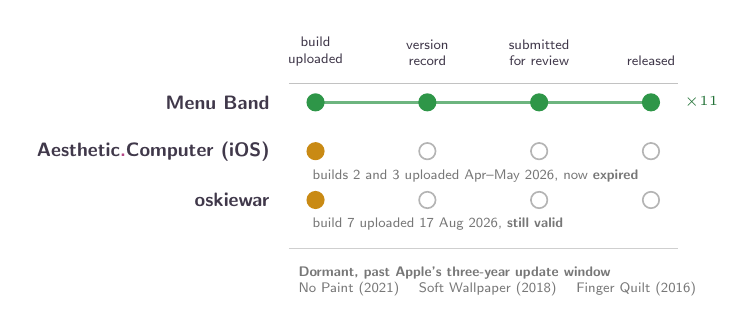
\begin{tikzpicture}[x=1cm, y=1cm]
% Stage matrix: rows are apps, columns are the four stages of Apple's
% release pipeline. A filled mark means the stage is complete. The claim
% is the shape of the bottom two rows, which stop at the first column.
\def\ca{0.00} \def\cb{1.42} \def\cc{2.84} \def\cd{4.26}
\def\ra{0.00} \def\rb{-0.62} \def\rc{-1.24}

% column headers
\foreach \cx/\h in {\ca/build\\uploaded, \cb/version\\record,
                    \cc/submitted\\for review, \cd/released}
  \node[font=\tiny\sffamily, text=acdark, anchor=south, align=center] at (\cx,0.34) {\h};
\draw[acgray!45, line width=0.4pt] (-0.34,0.24) -- (4.60,0.24);

% row labels
\node[font=\scriptsize\sffamily, text=acdark, anchor=east] at (-0.46,\ra) {\textbf{Menu Band}};
\node[font=\scriptsize\sffamily, text=acdark, anchor=east] at (-0.46,\rb) {\textbf{\ac{} (iOS)}};
\node[font=\scriptsize\sffamily, text=acdark, anchor=east] at (-0.46,\rc) {\textbf{oskiewar}};

% Menu Band: complete, eleven times
\draw[acgreen!70, line width=0.9pt] (\ca,\ra) -- (\cd,\ra);
\foreach \cx in {\ca,\cb,\cc,\cd}
  \node[circle, fill=acgreen, draw=acgreen, line width=0.6pt, inner sep=2.1pt] at (\cx,\ra) {};
\node[font=\tiny\sffamily, text=acgreen!75!black, anchor=west] at (4.56,\ra) {$\times11$};

% AC for iOS: stalls at stage one, builds expired
\node[circle, fill=acamber, draw=acamber, line width=0.6pt, inner sep=2.1pt] at (\ca,\rb) {};
\foreach \cx in {\cb,\cc,\cd}
  \node[circle, draw=acgray!55, line width=0.6pt, fill=white, inner sep=2.1pt] at (\cx,\rb) {};

% oskiewar: stalls at stage one, build still live
\node[circle, fill=acamber, draw=acamber, line width=0.6pt, inner sep=2.1pt] at (\ca,\rc) {};
\foreach \cx in {\cb,\cc,\cd}
  \node[circle, draw=acgray!55, line width=0.6pt, fill=white, inner sep=2.1pt] at (\cx,\rc) {};

% per-row notes, placed on their own line beneath each stalled row
\node[font=\tiny\sffamily, text=acgray, anchor=west] at (\ca-0.16,\rb-0.32)
  {builds 2 and 3 uploaded Apr--May 2026, now \textbf{expired}};
\node[font=\tiny\sffamily, text=acgray, anchor=west] at (\ca-0.16,\rc-0.30)
  {build 7 uploaded 17 Aug 2026, \textbf{still valid}};

% dormant set, ruled off below
\draw[acgray!35, line width=0.4pt] (-0.34,-1.86) -- (4.60,-1.86);
\node[font=\tiny\sffamily, text=acgray, anchor=north west, align=left] at (-0.34,-1.96)
  {\textbf{Dormant, past Apple's three-year update window}\\
   No Paint (2021) \quad Soft Wallpaper (2018) \quad Finger Quilt (2016)};
\end{tikzpicture}
\caption{Where each app sits in Apple's release pipeline. \emph{Menu Band} completes all four stages routinely. Two finished applications stop at the first, which is invisible to every customer and reversible in an afternoon.}
\label{fig:pipeline}
\end{figure}

\ac{} for iOS is the costly case. The App Store serves
version 1.0, released 4~July 2023. Two later builds were uploaded, on
23~April and 1~May 2026, and no version record was ever created for
them, so neither reached a single user. Both are now expired. The
repository shows what they contained: \texttt{apple/PROGRESS.md} records
build~2 as a push-notification rewrite and build~3 as a reliability pass
fixing a documented failure in which the app hangs on the boot animation
with no recovery short of force-quit, addressed with a watchdog timer, a
navigation-failure delegate, pull-to-refresh, and an offline retry path.
That fix exists, was tested, and is not in the hands of anyone who has
the app. Section~\ref{sec:runtime} shows how many people that is.

\emph{oskiewar} is the cheap case. A complete build was uploaded on
17~August 2026, it has not expired, and both the iOS and macOS version
records sit in \texttt{PREPARE\_FOR\_SUBMISSION}. The submission tooling
to finish it already exists and is proven: \texttt{bin/asc.mjs submit}
performs the whole last mile idempotently, and it was written for
\emph{Menu Band} precisely because doing it by hand across three resource
types in the wrong order leaves a version that looks ready and was never
sent.

The dormant three carry a deadline that is not self-imposed. Apple's App
Store Improvements process identifies for removal any app that has gone
three years without an update and falls below a minimum download
threshold over a rolling twelve months, with ninety days to
respond~\citep{apple2022improvements}. \emph{Finger Quilt} last shipped
in 2016, \emph{Soft Wallpaper} in 2018, \emph{No Paint} in 2021. All
three are past the update window, and whether they are past the download
threshold is unknown, because until 9~September 2026 no analytics report
existed for any of them to say. A removed app keeps working for people
who already have it and disappears for everyone else, which for
\emph{No Paint} would mean losing a ten-year listing carrying 131
reviews at 4.74 stars.

\section{What the Runtime Already Carries}
\label{sec:runtime}

The store is one distribution channel and the web is the other. Boot
telemetry lets the two be compared directly, because both surfaces load
the same runtime and both report.

\begin{table}[t]
\centering
\small
\caption{Monthly boots by surface in 2026. The iOS application is identified by its custom user agent together with handheld screen geometry. February is an unexplained web outlier and is excluded from typical-month reasoning. September is partial, covering nine days.}
\label{tab:boots}
\begin{tabularx}{\columnwidth}{@{}l r r X@{}}
\toprule
\textbf{Month} & \textbf{iOS app} & \textbf{iOS web} & \textbf{All web} \\
\midrule
2026-02 & 1{,}429 & 1{,}827 & 51{,}276 \\
2026-03 & 2{,}638 & 1{,}020 & 7{,}507 \\
2026-04 & 2{,}944 & 1{,}248 & 8{,}877 \\
2026-05 & 2{,}273 & 1{,}068 & 6{,}005 \\
2026-06 & 1{,}362 & 1{,}395 & 7{,}574 \\
2026-07 & 1{,}087 & \phantom{0}649 & 6{,}194 \\
2026-08 & 1{,}604 & 1{,}199 & 7{,}860 \\
2026-09 & \phantom{0}493 & \phantom{0}333 & 3{,}003 \\
\midrule
\textbf{Total} & \textbf{13{,}830} & \textbf{8{,}739} & \textbf{98{,}296} \\
\bottomrule
\end{tabularx}
\end{table}

Table~\ref{tab:boots} carries the argument for finishing the iOS
release. In every month of 2026 except February and June, the wrapped
iOS application produced more sessions than mobile Safari did. Over the
period it produced 13,830 handheld boots against 8,739 from iPhone and
iPad browsers. Whatever its store presence looks like, the app is a
live, load-bearing surface, and it is running a binary from July 2023
with a known hang whose fix expired in TestFlight.

The comparison also sets the scale honestly. Native sessions are about
one seventh of total web sessions. The store is a real but minority
channel, and the case for investing in it rests on what it uniquely
provides rather than on volume: a discovery surface that demonstrably
converts, a payment mechanism, a permanent listing, and access to system
capabilities the browser withholds.

\section{Openings}
\label{sec:openings}

Nine actions, ordered by evidence-to-effort. Each names the finding that
motivates it and the smallest test that would settle it.

\begin{enumerate}
\item \textbf{Finish \emph{oskiewar}'s macOS listing, then submit it.}
A finished, unexpired macOS build (build~7) has sat since 17~August 2026
against a version record in \texttt{PREPARE\_FOR\_SUBMISSION}, and the
submission tooling exists. Three things stand between it and review,
none of them a build: \texttt{asc.mjs} was written against \emph{Menu
Band}'s application identifier and the macOS platform, so it must be
told which app it is addressing; the store listing is empty on both
platforms, with \texttt{description}, \texttt{keywords} and
\texttt{supportUrl} all null and no screenshots attached; and build~7's
pre-release version records \texttt{MAC\_OS}, so it cannot serve the
iOS record beside it. The listing is the work, and it is an afternoon
of writing rather than an hour of shipping. \emph{This entry was
corrected after the audit: the first draft described the submission as
one command away, which the App Store Connect API does not support.}

\item \textbf{Build \emph{oskiewar} for iOS.} The iOS version record
has existed since 17~August 2026 with no build behind it. Until one is
archived and uploaded, the claim that \emph{oskiewar} supplies the
account's first iOS release since 2023 has nothing to stand on.

\item \textbf{Ship \ac{} for iOS 1.1.} 13,830 handheld
sessions run a three-year-old binary while its reliability fix expires
in TestFlight. Rebuild from the code documented in
\texttt{apple/PROGRESS.md}, create the version record, submit. The
app's one negative review complains about unwanted notifications, which
the build~2 push rework directly addresses.

\item \textbf{Return \emph{Menu Band} to \$4.99.} Every recorded sale
happened at \$4.99 and none at \$9.99. Change the price, wait four
weeks, read the analytics. If units resume, the finding is worth more
than the four dollars of margin.

\item \textbf{Update \emph{No Paint} before Apple removes it.} A
ten-year listing with 131 reviews at 4.74 stars sits five years past its
last release and inside the removal window. A minimal build that clears
the deployment target, adds a visible new-painting control and an undo
button, and points at the current \texttt{nopaint.art} redirect would
protect the asset and close the two usability complaints the review
corpus repeats.

\item \textbf{Instrument everything.} Four ONGOING analytics report
requests were created on 9~September 2026 for the apps that lacked them,
and their first instances land within days. Read them, and read the App
Downloads Standard report alongside purchases, so the download-threshold
half of the removal criterion stops being invisible.

\item \textbf{Recover the vendor number.} Sales and Trends gives
same-day exact units across the whole catalog, and it is blocked on one
value readable from the Payments and Financial Reports page in App Store
Connect. Everything commercial in this paper is currently limited by a
four-week backfill horizon that Sales and Trends does not have.

\item \textbf{Rebuild the referral path that worked.} The one demand
event in ten years came from short-video attention pointed at a free
drawing tool, and it decayed because nothing caught it. The catalog now
has an account system, a notification path, and a network to arrive
into. A store listing that leads into \ac{} rather than terminating in a
single app converts attention into membership.

\item \textbf{Treat the listing as the artifact.} Four of five
\emph{Menu Band} sales converted on the product page, and three of five
were discovered by Apple's own search and browse. That makes screenshots,
subtitle, and keywords the highest-leverage surface in the account, and
they are already generated from real UI by
\texttt{bin/app-store-real.mjs}. Extend that pipeline to the other apps
rather than writing new marketing.
\end{enumerate}

Items~1 through~5 are executable within a week and need no new code,
though item~1 needs a listing written and item~2 needs a build archived.
Items~6 and~7 are measurement. Items~8 and~9 are the strategy the first
seven make possible.

\section{Limitations}
\label{sec:limits}

The commercial record is incomplete at the front. The analytics backfill
horizon of 13~July 2026 means \emph{Menu Band} sales between its 7~May
launch and 12~July are unrecoverable through this route, so five units is
a floor rather than a total. Lifetime downloads for every app remain
unknown pending the vendor number.

Boot counts are page loads. A single enthusiastic session inflates them
the same way a hundred visitors would, and no per-user identity is
attached, so nothing here should be read as an audience size. The
February 2026 web figure of 51,276 is an outlier this paper does not
explain and does not use.

The price hypothesis rests on five transactions. It is stated as a test
to run rather than a conclusion, and it would be irresponsible to
describe it otherwise.

Reviews are a biased instrument everywhere, over-representing delight and
grievance and under-representing the ordinary middle. Their value here is
in the specific and repeated complaints, which are actionable regardless
of what the ratings mean.

Finally, the removal risk is a policy reading rather than a notice.
Apple's stated criteria are conjunctive, requiring both staleness and low
downloads~\citep{apple2022improvements}, and the download half is exactly
what has never been measured. No removal warning has been received for
any app in this account.

\section{Ethics and Privacy}
\label{sec:ethics}

Review text quoted here is public on the App Store. Reviewer nicknames
are omitted throughout, and quotations are limited to what supports a
stated finding. One low-rated review makes a professional allegation
about the developer; it is counted in the distribution and its content
is not reproduced, because it concerns conduct rather than software and
repeating it would neither test it nor answer it.

Boot telemetry is aggregate. No document is quoted, no handle is named,
and no geographic detail finer than a country is used. The runtime
collects this data to debug boot failures, and reusing it for a
distribution audit is a secondary use of records already held, which is
worth stating rather than assuming.

Commercial figures are the developer's own. The five transactions include
territory and discovery source as Apple reports them, and no purchaser is
identifiable from any field used here.

\section{Conclusion}
\label{sec:conclusion}

Ten years produced six app records, 152 reviews averaging 4.65 stars, one
demand event, and \$17.81.

The record's lesson is narrower than the numbers suggest. The work was
done. Three small iOS pieces shipped and found real affection, one of
them at a scale that briefly mattered. A menu-bar instrument received 420
commits and eleven releases in a single summer. A reliability fix for the
most-used native surface was written, tested, and documented. What
failed repeatedly was the conversion of finished software into
distribution, which on Apple's store is four administrative steps that
take an afternoon and are invisible when skipped. Two applications sit at
the first of those steps right now, and one of them serves nearly
fourteen thousand sessions a year with a binary from 2023.

The measurement failure compounds it. Until the day this audit began, no
analytics report existed for five of six apps, which meant the account
could not answer whether anything was being downloaded, could not see the
removal risk accumulating against its oldest and best-loved listing, and
could not have noticed a price change coinciding with the end of sales.
That is now fixed, and the first reports arrive within days.

The strategic finding is the one worth carrying forward. Attention has
never been the constraint. In 2020 it arrived unbidden and was allowed to
drain away, and in 2026 Apple's own search surface found buyers for an
unmarketed instrument three times out of five. The constraint is the last
mile, and the last mile is cheap.

\appendix

\section{Rating Distribution}
\label{sec:appendix}

Table~\ref{tab:ratings} is the full rating census behind the mean quoted
in Section~\ref{sec:record}. It is included because the mean alone
misleads: 4.65 stars across 152 reviews sounds like a normal
distribution centred high, and the actual shape is 133 five-star ratings,
nine one-star ratings, and ten reviews in between. Small-sample app
reviews behave this way generally, and the practical consequence is that
the middle of the scale carries almost no information here while the two
poles carry all of it. The nine one-star reviews were therefore read
individually rather than counted, and two of them produced the usability
items in opening~4.

\begin{table}[h]
\centering
\footnotesize
\caption{Rating census across all reviewed apps, pulled complete from the App Store Connect API on 9~September 2026. \emph{Menu Band} and \emph{oskiewar} have no reviews and are omitted.}
\label{tab:ratings}
\begin{tabularx}{\columnwidth}{@{}X r r r r r r r@{}}
\toprule
\textbf{App} & \textbf{1} & \textbf{2} & \textbf{3} & \textbf{4} & \textbf{5} & \textbf{N} & \textbf{Mean} \\
\midrule
No Paint         & 6 & 1 & 1 & 5 & 118 & 131 & 4.74 \\
Soft Wallpaper   & 2 & 0 & 2 & 0 & 13  & 17  & 4.29 \\
Finger Quilt     & 0 & 1 & 0 & 0 & 1   & 2   & 3.50 \\
\ac{} (iOS)      & 1 & 0 & 0 & 0 & 1   & 2   & 3.00 \\
\midrule
\textbf{Total}   & \textbf{9} & \textbf{2} & \textbf{3} & \textbf{5} & \textbf{133} & \textbf{152} & \textbf{4.65} \\
\bottomrule
\end{tabularx}
\end{table}

\bibliographystyle{plainnat}
\setlength{\bibsep}{1.6pt plus 0.3ex}
{\small
\bibliography{references}
}

\end{document}
